\documentclass[10pt,letterpaper]{article}
\usepackage[T1]{fontenc}
\usepackage{amssymb}
\usepackage{amsmath}
\usepackage{braket}
\usepackage{enumerate}
\usepackage[margin=0.5in]{geometry}
\usepackage{graphicx}
\usepackage{tabularx}
\usepackage{xcolor}
\title{Introduction to Quantum Electronic Devices and Applications}
\author{Jeremy Chen}
\date{14/04/2026}

\newcolumntype{P}[1]{>{\centering\arraybackslash}p{#1}}

\begin{document}
	\maketitle
	
\begin{enumerate}[\textbf{\arabic{enumi}.}]

\item \textbf{\textbf{Single Qubit Quantum Logic Gates}}

\begin{enumerate}[a)]

\item \textit{Pauli Gates}: Many single-qubit gates implement rotations around a particular axis. These include the Pauli-X, Pauli-Y, and Pauli-Z gates.

\begin{enumerate}[i.]

\item Plot the initial state $\ket{\psi} = \frac{1}{\sqrt{2}}\ket{0} + \frac{e^{\frac{i\pi}{4}}}{\sqrt{2}}\ket{1}$ on a Bloch sphere. 

\begin{figure}[h!]
\centering
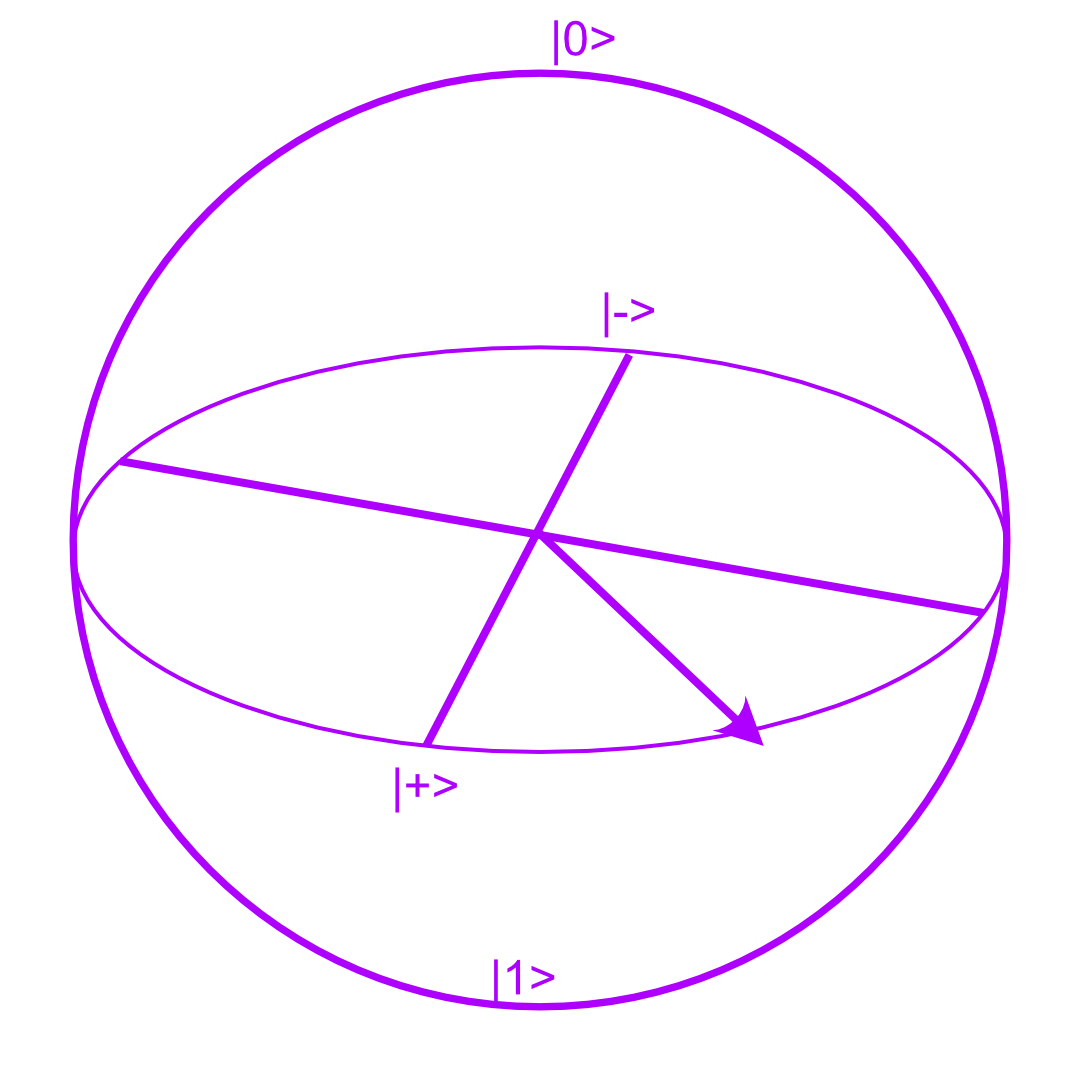
\includegraphics[width=200px]{BlochSphere}
\end{figure}

\item For each of the following gates $U$, calculate the resulting state $\ket{\psi'} = U\ket{\psi}$ and plot it along with the initial state $\ket{\psi}$ on the Bloch sphere to demonstrate the stated effect of the gate.

\textit{Hint}: to verify the rotation of the states, express all the output states in the form
$$\ket{\psi} = \alpha\ket{0} + \beta e^{i\varphi}\ket{1}$$

\begin{itemize}

\item Show that the Pauli-X gate rotates the initial state by $\pi$ radians around the x-axis. 

\color{violet}
Given some state $\ket{\psi}$, the alternative representation of its probability is $\ket{\psi} = \begin{bmatrix}
\alpha \\
\beta
\end{bmatrix}$. The Pauli-X gate is represented by matrix $\begin{bmatrix}
0 & 1 \\
1 & 0 
\end{bmatrix}$, so an operation on state $\ket{\psi}$ would be
\begin{gather*}
\ket{\psi'} = \begin{bmatrix}
0 & 1 \\
1 & 0 
\end{bmatrix}\begin{bmatrix}
\alpha \\
\beta 
\end{bmatrix} = \begin{bmatrix}
\beta \\
\alpha 
\end{bmatrix} \rightarrow \beta\ket{0} + \alpha e^{i\varphi}\ket{1}
\end{gather*}
Given that the initial state of the qubit is in $\ket{0}$, $\ket{\psi} = 1\ket{0} + 0\ket{1}$, the Pauli-X gate would give new state $\ket{\psi'} = 0\ket{0} + 1\ket{1}$. 
\color{black}

\item Show that the Pauli-Y gate rotates the initial state by $\pi$ radians around the y-axis. 

\color{violet}
The Pauli-Y gate is $\begin{bmatrix}
0 & -i \\
i & 0 
\end{bmatrix}$, so an operation would be
\begin{gather*}
\ket{\psi'} = \begin{bmatrix}
0 & -i \\
i & 0 
\end{bmatrix}\begin{bmatrix}
\alpha \\
\beta 
\end{bmatrix} = \begin{bmatrix}
-i\beta \\
i\alpha
\end{bmatrix} \rightarrow -i\beta\ket{0} + i\alpha e^{i\varphi}\ket{1}
\end{gather*}
Given an initial state $\ket{+} = \frac{1}{\sqrt{2}}\ket{0} + \frac{1}{\sqrt{2}}e^{i0}\ket{1}$, the new state would be $\ket{\psi'} = -i\frac{1}{\sqrt{2}}\ket{0} + i\frac{1}{\sqrt{2}}e^{i0}\ket{1}$ which is equivalent to $\frac{1}{\sqrt{2}}\ket{0} + \frac{1}{\sqrt{2}}e^{i\pi}\ket{1}$ or $\ket{-}$. 
\color{black}

\item Show that the Pauli-Z gate rotates the initial state by $\pi$ radians around the z-axis. 

\color{violet}
The Pauli-Z gate is $\begin{bmatrix}
1 & 0 \\
0 & -1 
\end{bmatrix}$, so an operation would be
\begin{gather*}
\ket{\psi'} = \begin{bmatrix}
1 & 0 \\
0 & -1 
\end{bmatrix}\begin{bmatrix}
\alpha \\
\beta 
\end{bmatrix} = \begin{bmatrix}
\alpha \\
-\beta
\end{bmatrix} \rightarrow \alpha\ket{0} - \beta\ket{1}
\end{gather*}
Given an initial state $\ket{+}$, the new state would be $\frac{1}{\sqrt{2}}\ket{0} - \frac{1}{\sqrt{2}}\ket{1}$, which is $\ket{-}$. 
\color{black}

\end{itemize}

\end{enumerate}

\item \textit{Hadamard Gate}: For the Hadamard gate $H$, determine the output state $\ket{\psi'}$ for the input states:

\begin{enumerate}[a.]

\item $\ket{\psi} = \ket{0}$

\color{violet}
The Hadamard gate is $\frac{1}{\sqrt{2}}\begin{bmatrix}
1 & 1 \\
1 & -1 
\end{bmatrix}$, so an operation on $\ket{0}$ would look like
\begin{gather*}
\ket{\psi'} = \frac{1}{\sqrt{2}}\begin{bmatrix}
1 & 1 \\
1 & -1
\end{bmatrix}\begin{bmatrix}
1 \\
0 
\end{bmatrix} = \frac{1}{\sqrt{2}}\begin{bmatrix}
1 \\
1 
\end{bmatrix} = \begin{bmatrix}
\frac{1}{\sqrt{2}} \\
\frac{1}{\sqrt{2}}
\end{bmatrix}
\end{gather*}
\color{black}

\item $\ket{\psi} = \ket{1}$

\color{violet}
For $\ket{1}$, an operation on $\ket{1}$ looks like
\begin{gather*}
\ket{\psi'} = \frac{1}{\sqrt{2}}\begin{bmatrix}
1 & 1 \\
1 & -1 
\end{bmatrix}\begin{bmatrix}
0 \\
1 
\end{bmatrix} = \frac{1}{\sqrt{2}}\begin{bmatrix}
1 \\
-1 
\end{bmatrix} = \begin{bmatrix}
\frac{1}{\sqrt{2}} \\
-\frac{1}{\sqrt{2}}
\end{bmatrix}
\end{gather*}
\color{black}

\end{enumerate}

What does the Hadamard gate do?

\color{violet}
The Hadamard gate puts a pure state into a mixed state with two possible outcomes for measurement, a superposition.
\color{black}

\item \textit{Phase Gate}: The phase gate $S$ is defined by the matrix $S = \begin{pmatrix}
1 & 0 \\
0 & i
\end{pmatrix}$. Apply the phase gate to the input state $\ket{\psi} = \frac{1}{\sqrt{2}}\ket{0} + \frac{1}{\sqrt{2}}\ket{1}$ to determine the output state $\ket{\psi'}$. What does the phase gate do?

\color{violet}
Given the matrix for a phase gate and an initial state, the new state would be
\begin{gather*}
\ket{\psi'} = \begin{bmatrix}
1 & 0 \\
0 & i 
\end{bmatrix}\begin{bmatrix}
\frac{1}{\sqrt{2}} \\
\frac{1}{\sqrt{2}} 
\end{bmatrix} = \begin{bmatrix}
\frac{1}{\sqrt{2}} \\
\frac{i}{\sqrt{2}} 
\end{bmatrix} \rightarrow \frac{1}{\sqrt{2}}\ket{0} + \frac{1}{\sqrt{2}}ie^{i0}\ket{1} = \frac{1}{\sqrt{2}}\ket{0} + \frac{1}{\sqrt{2}}e^{i\frac{\pi}{2}}\ket{1}
\end{gather*}
\color{black}

\end{enumerate}

\item \textbf{Multiple Qubit Quantum Logic Gates}

\begin{enumerate}[a)]

\item \textit{Hadamard Transform}: The Hadamard transform consists of Hadamard gates acting in parallel on multiple bits.

\begin{figure}[h!]
\centering
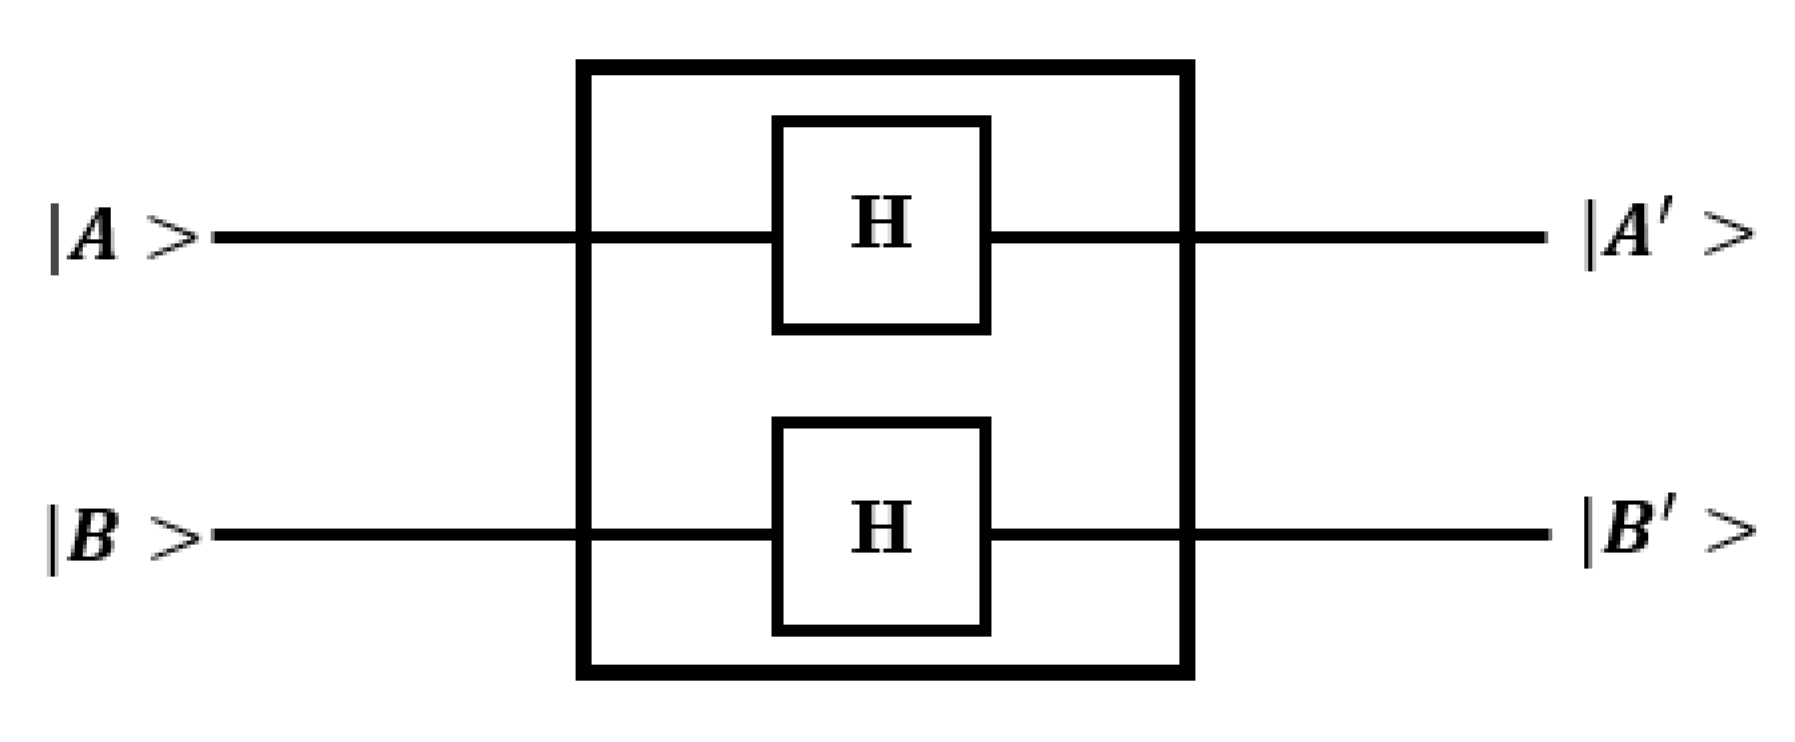
\includegraphics[width=200px]{2QubitHadamard}
\caption[]{\textit{2-Qubit Hadamard Transform}}
\end{figure}

Determine the output of the Hadamard transform for the input qubit states
$$\ket{A}\ket{B} = \ket{0}\ket{0}$$
Express your result as a superposition of 2-qubit states, for example:
$$\ket{A'B'} = \alpha_{00}\ket{00} + \alpha_{01}\ket{01} + \alpha_{10}\ket{10} + \alpha_{11}\ket{11}$$

\color{violet}
A Hadamard gate being applied to two qubits is an independent operation on each qubit state.
\begin{gather*}
\ket{A'} = \frac{1}{\sqrt{2}}\begin{bmatrix}
1 & 1 \\
1 & -1
\end{bmatrix}\begin{bmatrix}
1 \\
0 
\end{bmatrix} = \frac{1}{\sqrt{2}}\begin{bmatrix}
1 \\
1
\end{bmatrix} = \begin{bmatrix}
\frac{1}{\sqrt{2}} \\
\frac{1}{\sqrt{2}} 
\end{bmatrix}
\end{gather*}
$\ket{B'}$ would have the same result. The sum of their states would be tensor product of the two states, $\ket{A'} \otimes \ket{B'}$, which would be
\begin{gather*}
\ket{A'} \otimes \ket{B'} = \begin{bmatrix}
\frac{1}{\sqrt{2}} \\
\frac{1}{\sqrt{2}} 
\end{bmatrix} \otimes \begin{bmatrix}
\frac{1}{\sqrt{2}} \\
\frac{1}{\sqrt{2}} 
\end{bmatrix} = \begin{bmatrix}
\frac{1}{2} \\
\frac{1}{2} \\
\frac{1}{2} \\
\frac{1}{2} 
\end{bmatrix} \rightarrow \frac{1}{2}\ket{00} + \frac{1}{2}\ket{01} + \frac{1}{2}\ket{10} + \frac{1}{2}\ket{11}
\end{gather*}
\color{black}

\item \textit{Toffoli Gate}: the Toffoli gate acts as a CCNOT (or controlled-controlled-NOT gate), in which there are two control qubits, $\ket{A}$ and $\ket{B}$, and one target qubit, $\ket{C}$.

\begin{figure}[h!]
\centering
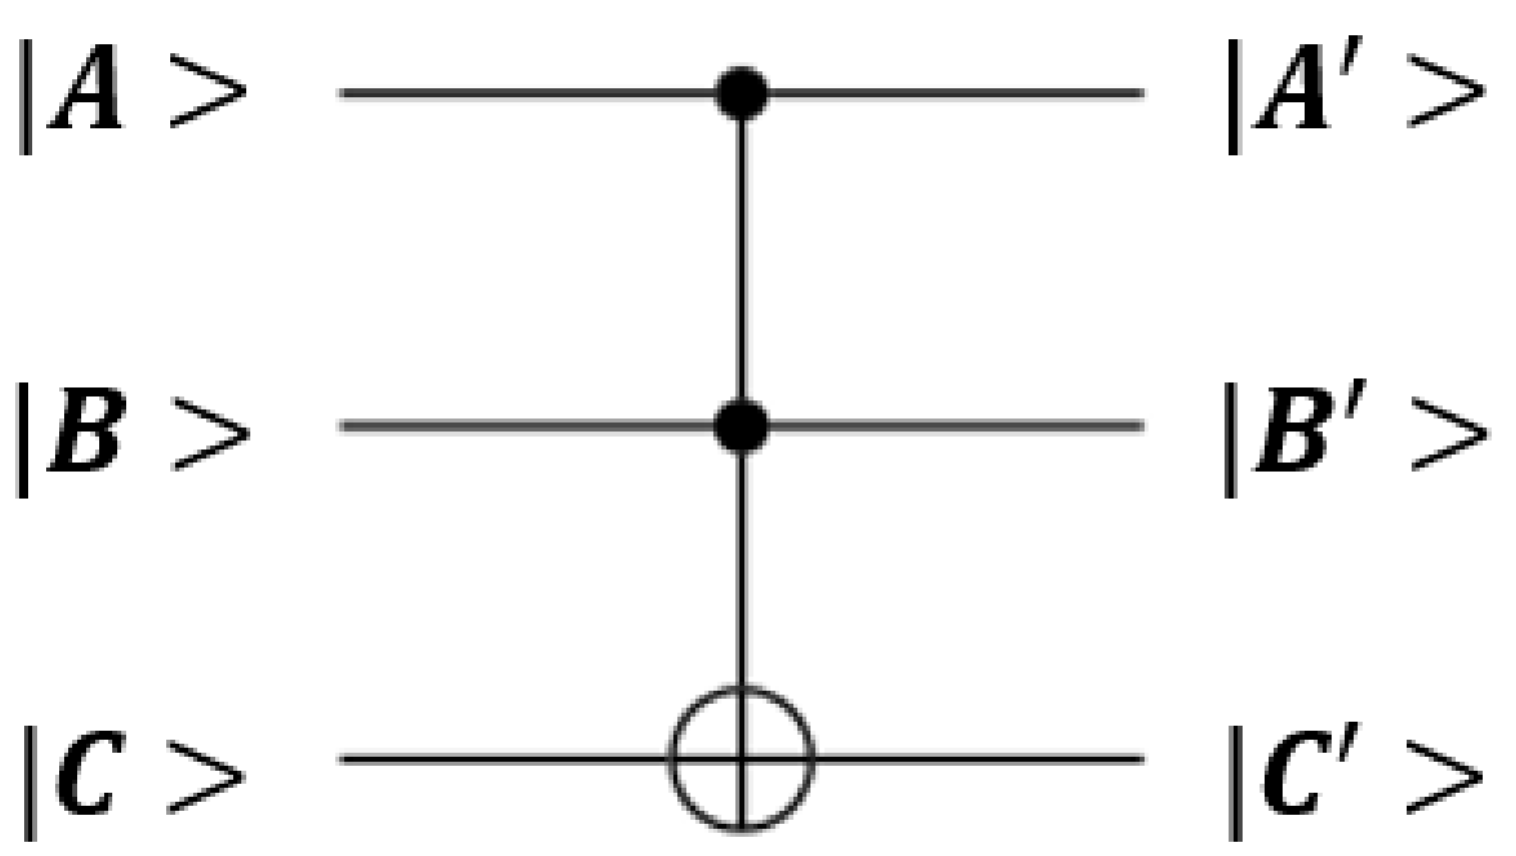
\includegraphics[width=150px]{ToffoliGate}
\caption{\textit{Toffoli Gate}}
\end{figure}

If the two control qubits are in state $\ket{1}$, then the target qubit will be flipped. Otherwise the target qubit's state remains unchanged. In all cases, the control qubit states do not change.

\begin{enumerate}[i.]

\item In classical computation, NAND gates are \textit{functionally complete}, meaning that any Boolean function can be implemented using a combination of NAND gates. As a result, we can build a classical computer using only NAND gates. Therefore, if we can to run classical algorithms on a quantum computer, it would be useful to be able to implement a classical NAND gate using quantum logic gates.

Generate a classical truth table for all possible input combinations to show that the Toffoli gate, with inputs as defined below, implements a reversible NAND gate. Explain how you can determine what the input qubit states were based on the output states (reversibility).

\begin{figure}[h!]
\centering
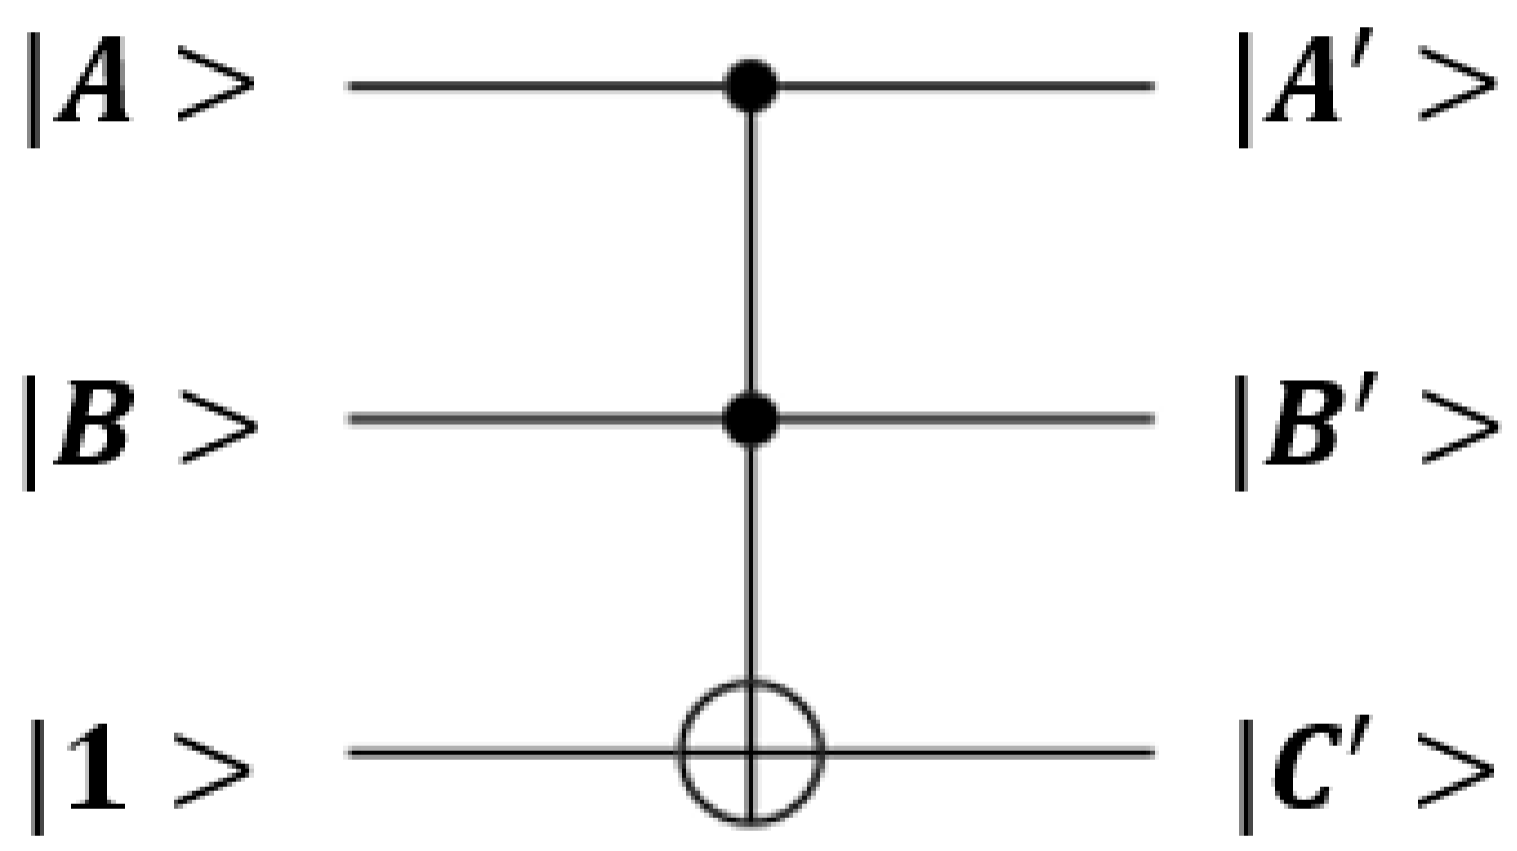
\includegraphics[width=150px]{RevNAND}
\caption{\textit{Reversible NAND Gate}}
\end{figure}

\color{violet}
Given the rules for a Toffoli gate, the following truth table shows the 8 possible states that a circuit could have
\begin{table}[h!]
\centering
\begin{tabular}{| P{0.5cm} | P{0.5cm} | P{0.5cm} | P{0.5cm} |}
\hline
$\ket{A}$ & $\ket{B}$ & $\ket{C}$ & $\ket{C'}$\\
\hline
0 & 0 & 0 & 0 \\
\hline
0 & 0 & 1 & 1 \\
\hline
0 & 1 & 0 & 0 \\
\hline
0 & 1 & 1 & 1 \\
\hline
1 & 0 & 0 & 0 \\
\hline
1 & 0 & 1 & 1 \\
\hline
1 & 1 & 0 & 1 \\
\hline
1 & 1 & 1 & 0 \\
\hline
\end{tabular}
\end{table}
The only state that changes is $\ket{C}$, so looking at $\ket{A}$, $\ket{B}$, and $\ket{C'}$ is sufficient in determining the input state. 
\color{black}

\item It is also useful in classical computation to take advantage of the \textit{fanout} operation, in which the value of a sinlge bit is distributed, or "copied" to different parts of the circuit. 

\begin{figure}[h!]
\centering
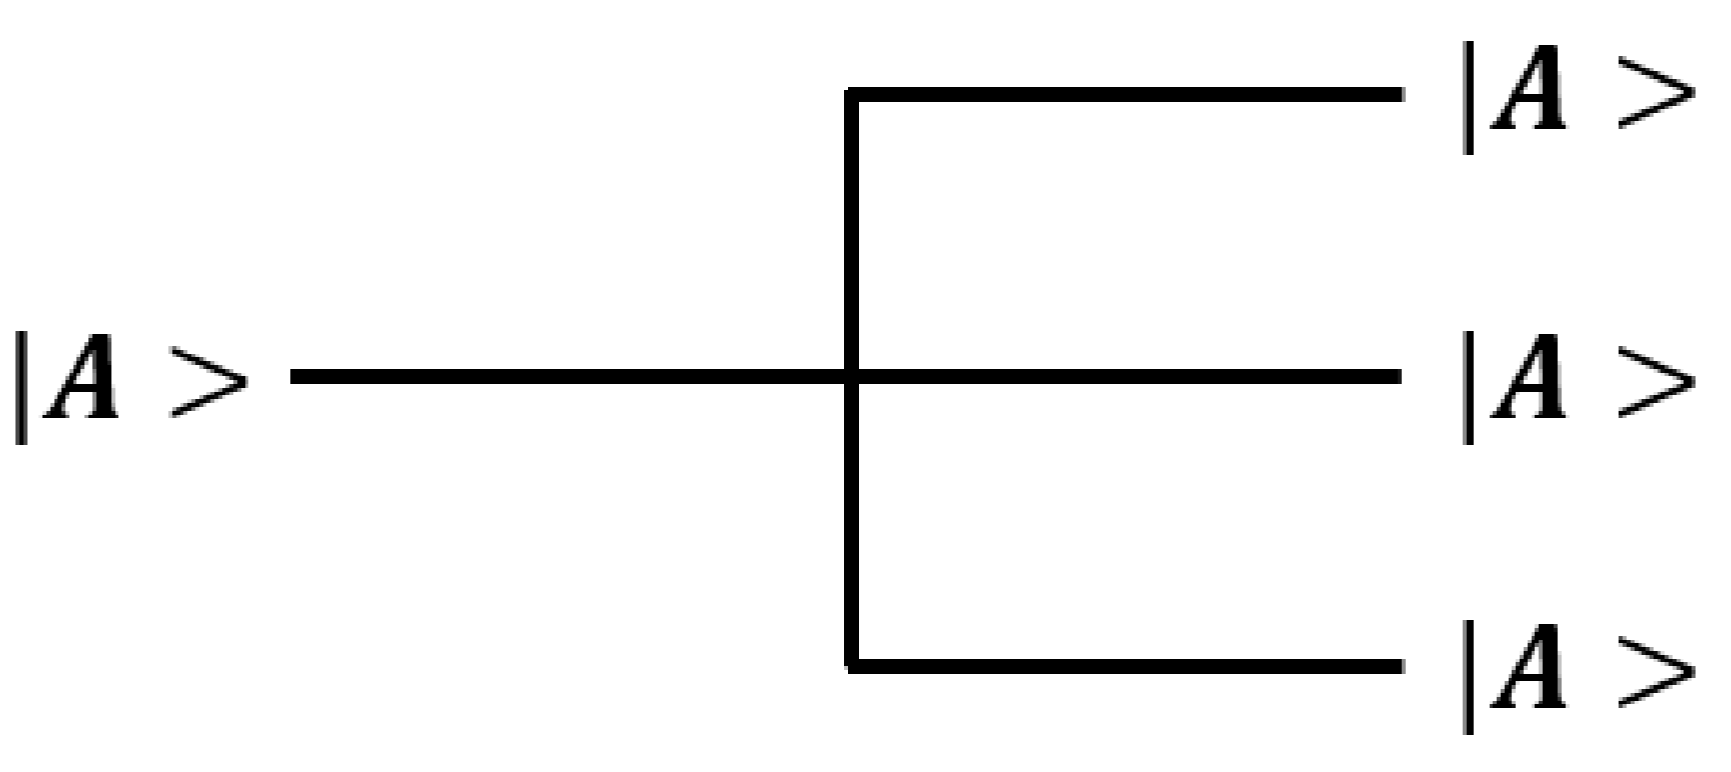
\includegraphics[width=200px]{ClassicalFanout}
\caption{\textit{Illustration of Classical Fanout}}
\end{figure}

When the inputs are properly configured as shown below, the Toffoli gate can also distribute the value of a single qubit to multiple wires of a quantum circuit.

\begin{figure}[h!]
\centering
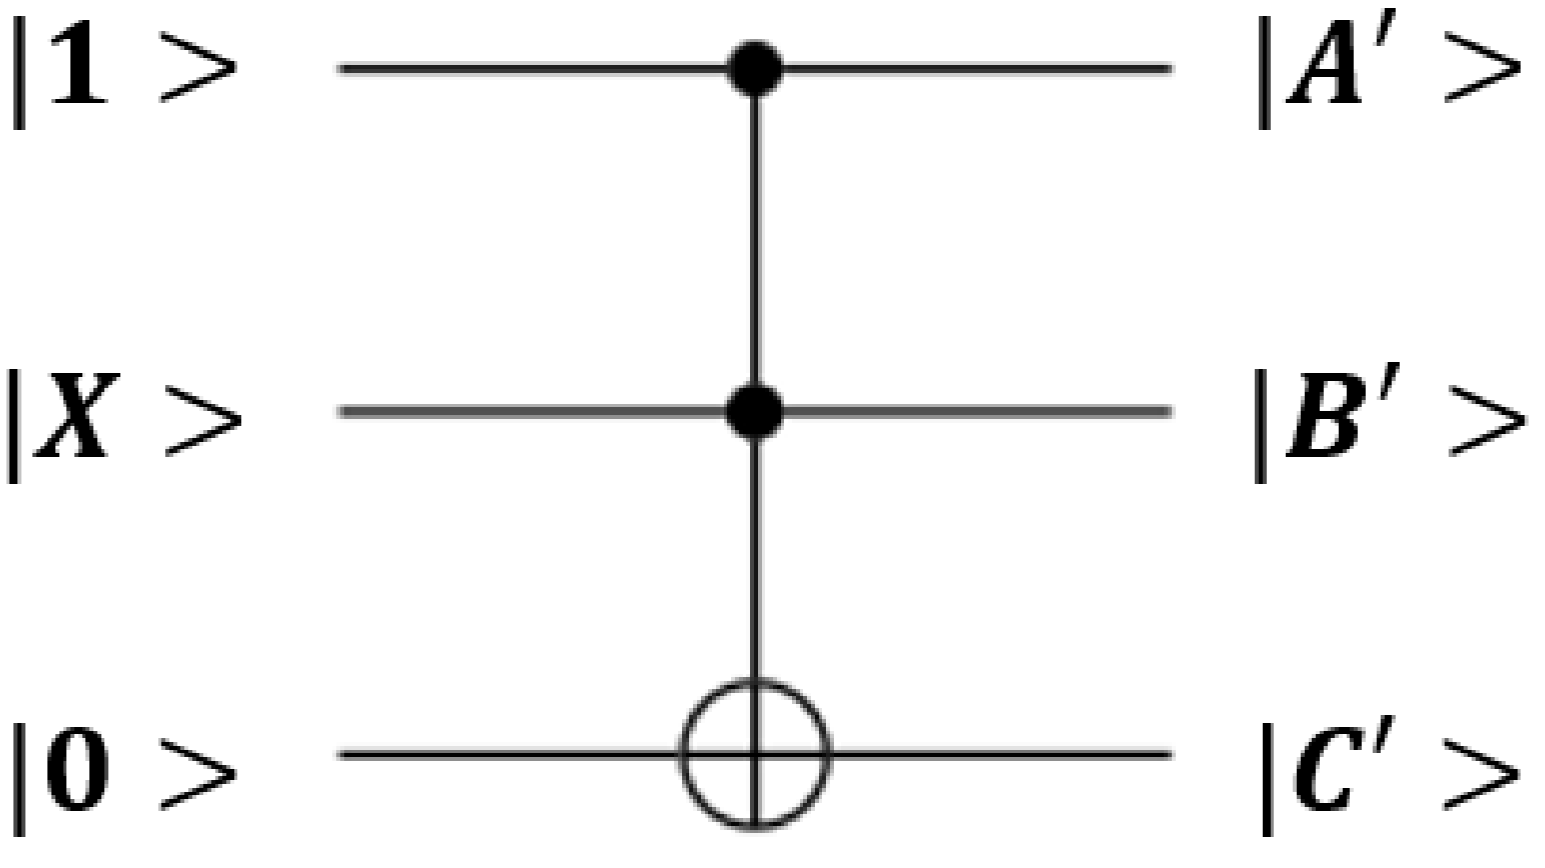
\includegraphics[width=150px]{ToffoliFanout}
\caption{\textit{Fanout Setup using a Toffoli Gate}}
\end{figure}

Generate a classical truth table for all possible input combination to show that the Toffoli gate, with inputs as defined above, distributes the state of qubit $\ket{X}$ to at least two output wires.

\textit{Note}: although we are "copying" the value of a single qubit's state, we are not necessarily copying the whole multi-qubit quantum state. This is forbidden in general by the "No-Cloning Theorem", which we will investigate in the next problem.

\color{violet}
The following truth shows all the possible values of $\ket{X}$ that gets distributed to $\ket{C}$. 
\begin{table}[h!]
\centering
\begin{tabular}{| P{0.5cm} | P{0.5cm} | P{0.5cm} | P{0.5cm} |}
\hline
$\ket{A}$ & $\ket{B}$ & $\ket{C}$ & $\ket{C'}$ \\
\hline
1 & 0 & 0 & 0 \\
\hline
1 & 1 & 0 & 1 \\
\hline
\end{tabular}
\end{table}
As seen here, the value of $\ket{C'}$ is dependent on $\ket{B}$, hence the distribution action. 
\color{black}

\item \textit{Extra Credit}: Implement each of your circuits from parts a) and b) in IBM's Quantum Composer or Qiskit. Show your results by including a screenshot of your circuit and plot Probability (\%) vs. Computational Basis States for each.

\textit{Note}: for b.i) and b.ii), you should show a circuit and results for each set of possible input states.

\end{enumerate}

\end{enumerate}

\item \textbf{Swap Circuit}

The quantum circuit below consists of 3 CNOT gates in series and implements a swap operation.

\begin{figure}[h!]
\centering
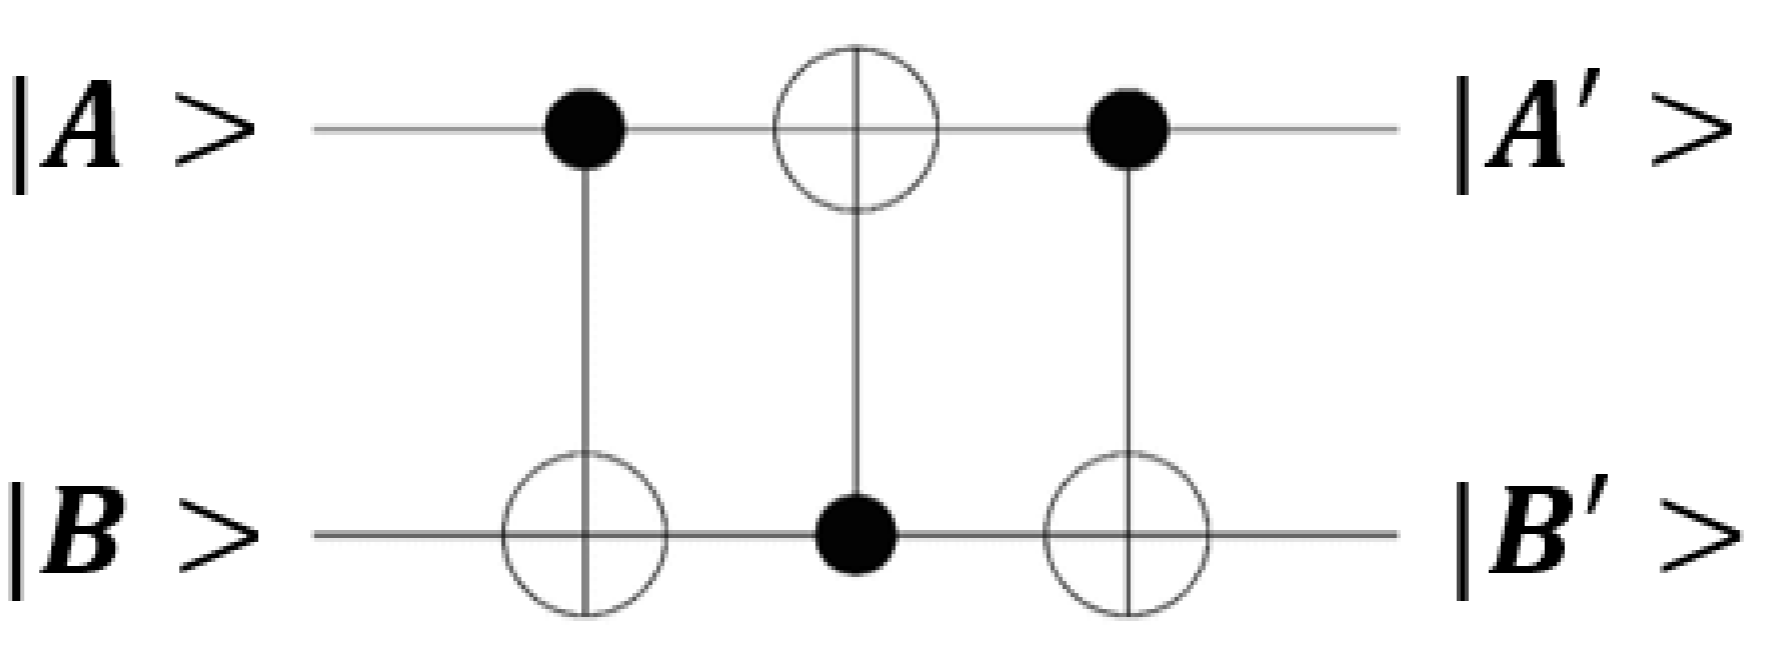
\includegraphics[width=200px]{Swap}
\caption{\textit{Swap Circuit}}
\end{figure}

\begin{enumerate}[a)]

\item Using the input state
$$\ket{\psi} = \alpha_{00}\ket{00} + \alpha_{01}\ket{01} + \alpha_{10}\ket{10} + \alpha_{11}\ket{11}$$
show that the output state of the swap circuit is
$$\ket{\psi'} = \alpha_{00}\ket{00} + \alpha_{10}\ket{01} + \alpha_{01}\ket{10} + \alpha_{11}\ket{11}$$
\textit{Hint}: although the first and third CNOT gates are in the usualy orientation such that $\ket{A}$ is the control qubit and $\ket{B}$ is the target qubit, the second CNOT gate's control and target qubit definitions are flipped and require a different gate matrix:
$$CNOT' = \begin{pmatrix}
1 & 0 & 0 & 0 \\
0 & 0 & 0 & 1 \\
0 & 0 & 1 & 0 \\
0 & 1 & 0 & 0
\end{pmatrix}$$ 

\color{violet}
Given the input state $\ket{\psi}$, the swap gate operation would look like
\begin{gather*}
CNOT\left( CNOT' \left( CNOT\left( \begin{bmatrix}
\alpha_{00} \\
\alpha_{01} \\
\alpha_{10} \\
\alpha_{11} 
\end{bmatrix} \right) \right) \right) = CNOT\left( CNOT'\left( \begin{bmatrix}
\alpha_{00} \\
\alpha_{01} \\
\alpha_{11} \\
\alpha_{10} 
\end{bmatrix} \right) \right) = CNOT\left( \begin{bmatrix}
\alpha_{00} \\
\alpha_{10} \\
\alpha_{11} \\
\alpha_{01} 
\end{bmatrix} \right) = \begin{bmatrix}
\alpha_{00} \\
\alpha_{10} \\
\alpha_{01} \\
\alpha_{11} 
\end{bmatrix} \\
\rightarrow \alpha_{00}\ket{00} + \alpha_{10}\ket{01} + \alpha_{01}\ket{10} + \alpha_{11}\ket{11}
\end{gather*}
\color{black}

\item Consider the initial state
$$\ket{\psi} = \frac{1}{\sqrt{2}}\ket{0}_{A}\ket{0}_{B} + \frac{1}{\sqrt{2}}\ket{0}_{A}\ket{1}_{B} = \frac{1}{\sqrt{2}}\ket{00} + \frac{1}{\sqrt{2}}\ket{01}$$
If we were to measure this state before sending it to the swap circuit, what are all of the possible measurement outcomes for each qubit ($A$ and $B$) and what are their corresponding probabilities?

\color{violet}
The possible measurement outcomes are $\ket{00}$ and $\ket{01}$, with probabilities $\frac{1}{2}$ for each qubit state. 
\color{black}

\item We send the initial state $\ket{\psi}$ from b) into the swap circuit. Calculate the output state $\ket{\psi'}$, then list all of the possible measurement outcomes for each qubit ($A'$ and $B'$) and their corresponding probabilities.

\color{violet}
The swap gate, given the outcome in part a), could be simplified to the matrix $\begin{bmatrix}
1 & 0 & 0 & 0 \\
0 & 0 & 1 & 0 \\
0 & 1 & 0 & 0 \\
0 & 0 & 0 & 1 
\end{bmatrix}$, which when given the initial state would result in $\ket{\psi'}$ of the following
\begin{gather*}
\begin{bmatrix}
1 & 0 & 0 & 0 \\
0 & 0 & 1 & 0 \\
0 & 1 & 0 & 0 \\
0 & 0 & 0 & 1 
\end{bmatrix}\begin{bmatrix}
\frac{1}{\sqrt{2}} \\
\frac{1}{\sqrt{2}} \\
0 \\
0 
\end{bmatrix} = \begin{bmatrix}
\frac{1}{\sqrt{2}} \\
0 \\
\frac{1}{\sqrt{2}} \\
0 
\end{bmatrix} \rightarrow \frac{1}{\sqrt{2}}\ket{00} + \frac{1}{\sqrt{2}}\ket{10}
\end{gather*}
\color{black}

\item Considering your results from b) and c), explain what the \textit{swap} operation actually does the the states of the qubits $A$ and $B$.

\color{violet}
It changes the states such that $\ket{01}$ and $\ket{10}$ swap their probabilities. 
\color{black}

\item \textit{Extra Credit}: Implement the swap circuit in IBM's Quantum Composer or Qiskit, using the initial state as defined in b) as the input. Verify the circuit's function by comparing its output to your answers for measurement probabilities in parts b) and c). Do this by adding measurement blocks to your circuit and plotting the Probability (\%) vs. Computational Basis States. Be sure to include screen shots of your circuit for each step as well.

\end{enumerate}

\item \textbf{The No-Cloning Theorem}

We saw in Problem 2 that a Toffoli gate can be used to distribute the state of a single qubit to multiple outputs. However, unlike in classical computing, we cannot \textit{copy} or \textit{clone} an entire, arbitrary quantum state and distribute it to different parts of the circuit; this is known as the \textit{No-Cloning Theorem} and provides constraints on quantum circuit and algorithm design. We will investigate this using the CNOT gate. 

\begin{enumerate}[a)]

\item Via a classical truth table, show that the CNOT gate, which the inputs as defined below, copies the state of qubit $X$ to both outputs $A'$ and $B'$.

\begin{figure}[h!]
\centering
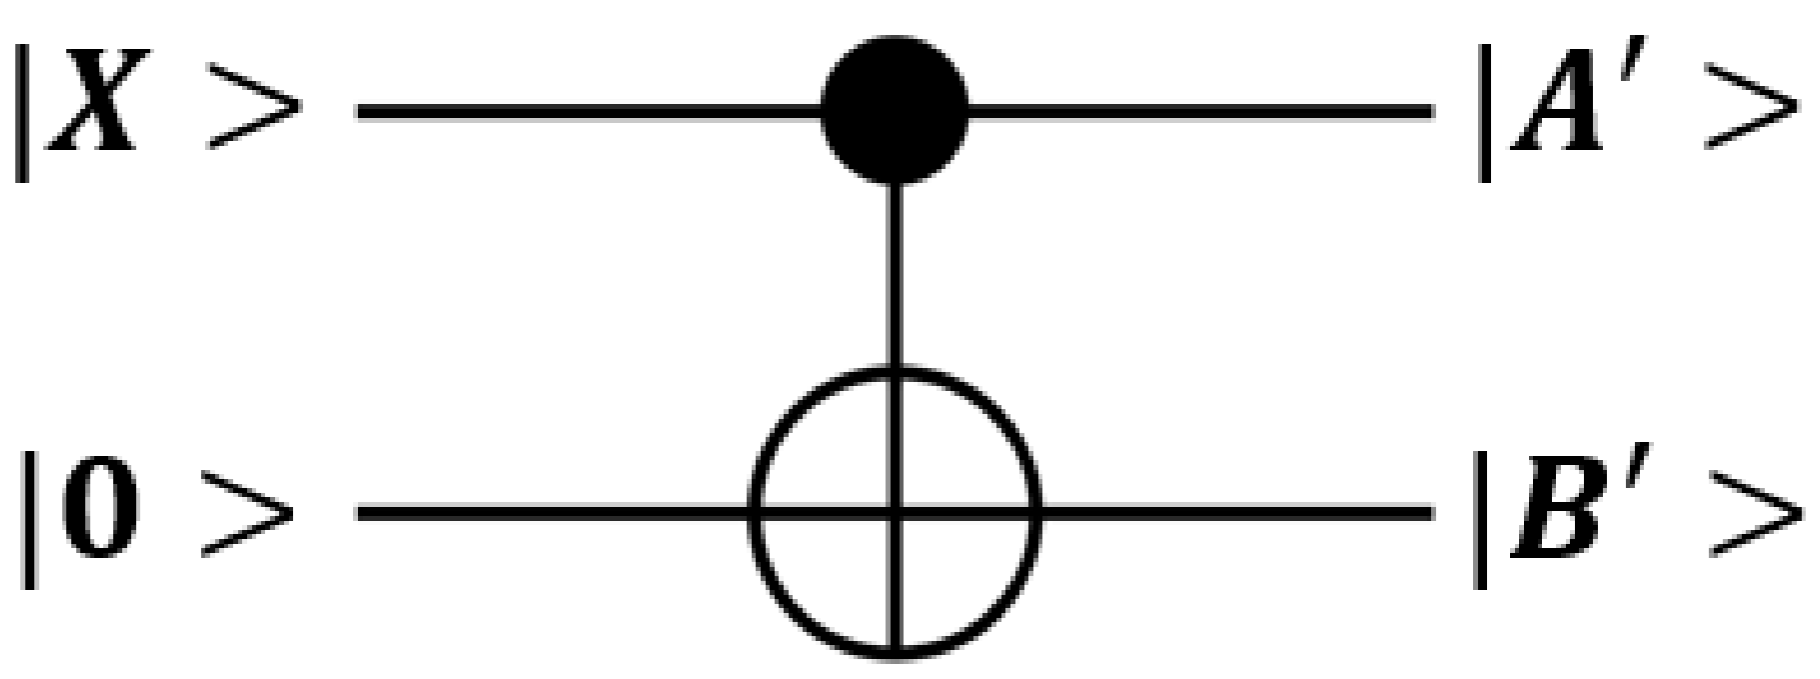
\includegraphics[width=200px]{CNOTFanout}
\caption{\textit{CNOT gate configured for fanout}}
\end{figure}

\color{violet}
The following truth table shows that when given an input to $\ket{X}$, both $\ket{A'}$ and $\ket{B'}$ will reflect that input.
\begin{table}[h!]
\centering
\begin{tabular}{| P{0.5cm} | P{0.5cm} | P{0.5cm} |}
\hline
$\ket{X}$ & $\ket{0}$ & $\ket{B'}$ \\
\hline
0 & 0 & 0 \\
\hline
1 & 1 & 1 \\
\hline
\end{tabular}
\end{table}
\color{black}

\item In order to actually \textit{clone} a state, we would need to input an initial state $\ket{\psi}$ and generate the output state $\ket{\psi'} = \ket{\psi} \otimes \ket{\psi}$.

For the initial state $\ket{X} = \ket{0}$, first, calculate the output state $\ket{\psi'} = \ket{X} \otimes \ket{X}$ that would result if we were to successfully clone the initial state. Next, calculate the output state the results from inputting $\ket{X} = \ket{0}$ into the CNOT gate as shown in (a). Does the CNOT gate successfully clone the state $\ket{X}$?

\color{violet}
If $\ket{X} = \ket{0}$, then the tensor product of two $\ket{X}$ would have result
\begin{gather*}
\ket{\psi'} = \begin{bmatrix}
1 \\
0 
\end{bmatrix} \otimes \begin{bmatrix}
1 \\
0 
\end{bmatrix} = \begin{bmatrix}
1 \\
0 \\
0 \\
0 
\end{bmatrix} \rightarrow \ket{00}
\end{gather*}
Likewise, if the input to the CNOT gate were $\ket{X}$, it would result in
\begin{gather*}
CNOT\left( \begin{bmatrix}
1 \\
0 \\
0 \\
0 
\end{bmatrix} \right) = \begin{bmatrix}
1 \\
0 \\
0 \\
0 
\end{bmatrix} \rightarrow \ket{00}
\end{gather*}
This shows that the CNOT managed to successfully clone the state $\ket{X}$. 
\color{black}

\item This time, consider the state $\ket{X} = \frac{1}{\sqrt{2}}\ket{0} + \frac{1}{\sqrt{2}}\ket{1}$. Calculate the output state if we were to successfully clone the initial state: $\ket{\psi'} = \ket{X} \otimes \ket{X}$. Then, calculate the output state the results from inputting $\ket{X}$ into the CNOT gate in (A). Does the CNOT gate successfully clone the state $\ket{X}$ in this case?

\color{violet}
The tensor product of the two states would result in
\begin{gather*}
\ket{\psi'} = \begin{bmatrix}
\frac{1}{\sqrt{2}} \\
\frac{1}{\sqrt{2}}
\end{bmatrix} \otimes \begin{bmatrix}
\frac{1}{\sqrt{2}} \\
\frac{1}{\sqrt{2}} 
\end{bmatrix} = \begin{bmatrix}
\frac{1}{2} \\
\frac{1}{2} \\
\frac{1}{2} \\
\frac{1}{2} 
\end{bmatrix}
\end{gather*}
Then, attempting that with a CNOT gate would get
\begin{gather*}
CNOT\left( \begin{bmatrix}
\frac{1}{\sqrt{2}} \\
\frac{1}{\sqrt{2}} 
\end{bmatrix} \otimes \begin{bmatrix}
1 \\
0 
\end{bmatrix} \right) = CNOT\left( \begin{bmatrix}
\frac{1}{\sqrt{2}} \\
0 \\
\frac{1}{\sqrt{2}} \\
0 
\end{bmatrix} \right) = \begin{bmatrix}
\frac{1}{\sqrt{2}} \\
0 \\
0 \\
\frac{1}{\sqrt{2}} 
\end{bmatrix}
\end{gather*}
which is not the same quantum state. Hence, the CNOT did not clone that state. 
\color{black}

\item What you should find is that the \textit{No-Cloning Theorem} does not forbid the cloning of all quantum states, but it forbids the cloning of \textit{arbitrary} quantum states. Based on your findings in (b) and (c), describe the circumstances under which we \textit{can} clone a quantum state and why those circumstances prevent us from assuming we can clone \textit{any} quantum state.

\color{violet}
Only pure states could be cloned, not mixed states. The superposition of the mixed states makes the transfer imperfect. 
\color{black}

\end{enumerate}

\end{enumerate}
	
\end{document}